\documentclass{article}

\usepackage[margin=0.5in]{geometry}
\usepackage{multicol}
\usepackage{tikz}
\usepackage{amsthm}

\theoremstyle{definition}
\newtheorem*{solution}{Solution}
\title{Problem-Solving Set B}
\author{}
\date{}

\begin{document}
\maketitle
\begin{multicols}{2}
    \begin{enumerate}
        \item Michelle teaches on Tuesday and Thursday evenings.
            On Tuesdays she makes $\$112.50$, and on Thursdays she makes $\$135$.
            There are $31$ days this month.
            What is the minimum amount that Michelle will earn this month?
            \begin{solution}
                Michelle will earn the minimum amount when there are only four Tuesdays and only four Thursdays during the $31$-day month.
                That will happen, for example, if the month starts on a Friday and ends on a Sunday.
                When that happens, Michelle will earn $4 \cdot 112.50 + 4 \cdot 135 = \$ 990$ or $\$ 990.00$.
            \end{solution}
        \item In a survey of $200$ people, $161$ reported owning a car, $58$ owned a bicycle, and $74$ had a valid mass transit pass.
            A total of $12\%$ of the survey respondents reported owning all three, while $2.5\%$ reported owning none.
            How many of the people surveyed owned exactly one of the three?
            \begin{solution}
                Of the $200$ survey respondents, $12\%$, or $200 \cdot 0.12 = 24$ people, reported owning a car, a bicycle, and a valid mass transit pass, while $2.5\%$, of $200 \cdot 0.025 = 5$ people, reported owning none of these.
                The Venn diagram shown summarizes what we know about the survey respondents.
                We let $A$, $B$, and $C$ represent the numbers of people who own a car, bicycle, and mass transit pass, respectively.
                Our ultimate goal is to find $A + B + C$, which is the number of people who won exactly one of the three.
                Next, we let $D$, $E$, and $F$ represent people who own a car, and a bicycle, a bicycle and a mass transit pass, and a car and a mass transit pass, respectively.
                Combined, the $161$ car owners, $58$ bicycle owners, and $74$ mass transit pass owners equal $161 + 58 + 74 = 293$ people.
                This total, however, counts the intersection of each pair of groups twice, and counts the intersection of all three groups three times.
                So, we have $A$ pair of groups twice, and counts the intersection of all three groups three times.
                So, we have $A + B + C+ 2(D + E + F) + 72 = 293$, which simplifies to $A + B + C + 2(D + E + F) = 221$.
                We also know that $A + B + C + D + E + F + 24 + 5 = 200$, which simplifies to $A + B + C + D + E + F = 171$.
                The difference between these two equations is $D + E + F = 221 - 171 = 50$.
                Substituting this back into $A + B + C + D + E + F = 171$, we find that $A + B + C + 50 = 171$, so $A + B + C = 121$.
                Therefore, the number of people who own exactly one of the three is $121$ people.
                \begin{center}
                    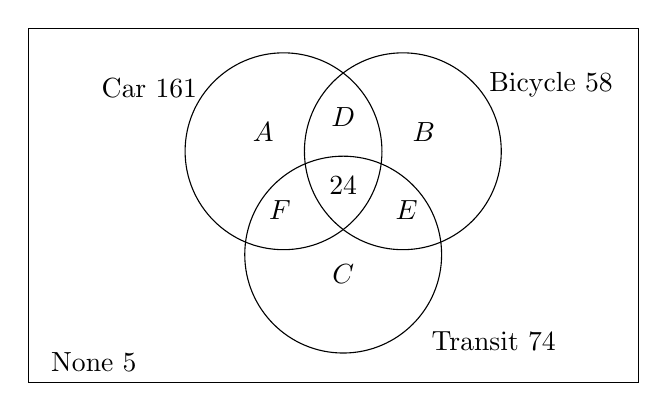
\begin{tikzpicture}[scale=0.5]
                        \draw (-8,-5) rectangle (7.5,4);
                        \draw(30:1.75cm) circle (2.5cm) node[above right]{$B$};
                        \draw(150:1.75cm) circle (2.5cm) node[above left]{$A$};
                        \draw(270:1.75cm) circle (2.5cm) node[below]{$C$};
                        \draw(90:1.25cm) node[above]{$D$};
                        \draw(-30:1.25cm) node[right]{$E$};
                        \draw(210:1.25cm) node[left]{$F$};
                        \draw(0,0) node{$24$};
                        \draw(30:4cm) node[above right]{Bicycle $58$};
                        \draw(150:4cm) node[above left]{Car $161$};
                        \draw(300:4cm) node[below right]{Transit $74$};
                        \draw(-5,-4) node[below left]{None $5$};
                    \end{tikzpicture}
                \end{center}
            \end{solution}
        \item Armin's $13$th birthday was on Saturday, July 4, 2020.
            How old will Armin be when his birthday next falls on a Saturday?
            \begin{solution}
                Since $365$ is one more than a multiple of $7$, the day of the week of Armin's birthday will shift one day forward each regular year and two days forward during a leap year (except in $2020$, since his birthday occurs after February 29, 2020).
                The table shows the day of Armin's birthday in the $6$ years it takes for his birthday to again be on a Saturday.
                Armin's birthday will next bon a Saturday when he is $13 + 6 = 19$ years old.
                \begin{center}
                    \begin{tabular}{|c|c|c|c|c|c|}
                        \hline
                        $2021$ & $2022$ & $2023$ & $2024$ & $2025$ & $2026$ \\
                        \hline
                        SUN & MON & TUE & THU & FRI & SAT \\
                        \hline
                    \end{tabular}
                \end{center}
            \end{solution}
        \item Tonya found $\$2.25$ in nickels and quarters in her sofa cushions.
            If the number of nickels Tonya found is five more than three times the number of quarters she found, what is the total number of coins Tonya found?
            \begin{solution}
                Let $n$ and $q$ represent the numbers of nickels and quarters, respectively, that Tonya found.
                We know that $0.05n + 0.25q = 2.25$, or $n + 5q = 45$.
                We also know that $n = 3q + 5$.
                Substituting for $n$ in the first equation, we get $3q + 5 + 5q = 45 \Rightarrow 8q + 5 = 45 \Rightarrow 8q = 40 \Rightarrow q = 5$.
                So, $n = 3q + 5 = 3 \cdot 5 + 5 = 20$.
                Tonya found $5$ quarters and $20$ nickels, for a total of $5 + 20 = 25$ coins.
            \end{solution}
        \item In how many ways can all the numbers $1$, $2$, $3$, $4$, $5$, $6$ and $7$ be separated into two groups, so that the sum of the numbers in both groups is the same?
            \begin{solution}
                The sum of all seven numbers is $28$, so we are looking for ways to create two groups, with the numbers of each grouped adding to $28 \div 2 = 14$.
                The group containing the $7$ must have the remaining numbers sum to $14 - 7 = 7$.
                The only ways to do this are $6 + 1$, $5 + 2$, $5 + 3$, and $4 + 2 + 1$.
                Therefore, the number of ways to separate the given numbers into two groups so that the sum of the numbers in each group is the same is $4$ ways.
            \end{solution}
    \end{enumerate}
\end{multicols}
\end{document}